\documentclass{article}

\usepackage[a4paper]{geometry}
\usepackage{lipsum}
\usepackage{graphicx}

\title{Project plan}
\author{Darcy Geyer, Sarah McCauley, Tin Nam Choi}
\date{2022\\October}

\begin{document}
  \maketitle{}
  
  \tableofcontents{}
  
  \pagebreak
  
  \section{Description}
  A turn-based role-playing Pokémon™ fighting game. 
  
  \lipsum[1]
  
  \pagebreak

  \section{Potential classes}
  
  \subsection{Player}
  Data: 
  \begin{itemize}
    \item Pokemon owned
    \item Level 
  \end{itemize}
  Functions:
  \begin{itemize}
    \item Add/remove Pokemon owned
    \item Increment/decrement level
  \end{itemize}
  
  \subsubsection{Person}
  Data:
  \begin{itemize}
    \item Name
    \item Skill points (for leveling up)
  \end{itemize}
  Functions:
  \begin{itemize}
    \item Set name
    \item Increment/decrement skill points
    \item Get action from user
  \end{itemize}
  
  \subsubsection{Computer}
  Functions:
  \begin{itemize}
    \item Get action randomly
  \end{itemize}
    
  \subsection{Pokemon}
  Data:
  \begin{itemize}
    \item Name
    \item Type
    \item Level
    \item Health
    \item Attack
    \item Defense
    \item Speed
    \item Moves learnt
  \end{itemize}
  Functions:
  \begin{itemize}
    \item Increment/decrement level
    \item Increment/decrement health
    \item Increment/decrement attack
    \item Increment/decrement defense
    \item Increment/decrement speed
    \item Add/remove moves learnt
  \end{itemize}
  
  \subsection{Menu}
  Data:
  \begin{itemize}
    \item Title
    \item Options (vector)
  \end{itemize}
  Functions:
  \begin{itemize}
    \item Print menu
    \item Set title
    \item Set options
  \end{itemize}
  
  \pagebreak
  
  \section{Timeline}
  
  \subsection*{Mid-term break}
  \begin{itemize}
    \item Finalize plan
    \item Prototypical testing
  \end{itemize}
  
  \subsection*{Week 9}
  \begin{itemize}
    \item Submit plan
    \item Begin coding
  \end{itemize}
  
  \subsection*{Week 10}
  \begin{itemize}
    \item Finish version 1
  \end{itemize}
  
  \subsection*{Week 11}
  \begin{itemize}
    \item Finish coding
  \end{itemize}
  
  \pagebreak
  
  \section{User interface}
  
  The game will use a command-line interface. This will be done using the Menu class to display the options to the user, and the user will be able to select an option by typing the corresponding number. 
  
  \begin{center}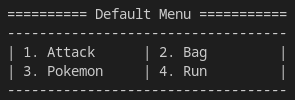
\includegraphics[height=2cm]{media/Menu.png}\end{center}
  
  \section{Testing and debugging plan}
  
  \lipsum[1-2]
  
\end{document}
